% Hauptdokument

% Definition von globalen Parametern und eigenen Kommandos

\newcommand{\praktikumTitel}{PSE 2012}
\newcommand{\projektTitel}{OQAT }
\newcommand{\dAU}{Bob } %Name für Scenarien

% Nummerierung für Muss-, Wunsch- und Abgrenzkriterien /MK-10/, /MK-20/, ...
% usage:
% \nItem{argument}
% results in : /argument-countervalue/
\newcounter{counterKriterien}
\newcommand{\nItem}[1]{\ \newline
\stepcounter{counterKriterien}/#1-\arabic{counterKriterien}0/ }
%Seiten- und Dokumentenlayout Einstellungen

\documentclass[
	11pt,								% Schriftgr��e
	DIV12,
	german,								% f�r Umlaute, Silbentrennung etc.
	oneside,							% einseitiges Dokument
	titlepage,							% es wird eine Titelseite verwendet
	halfparskip,						% Abstand zwischen Abs�tzen (halbe Zeile)
	normalheadings,						% Gr��e der �berschriften verkleinern
	tablecaptionabove,					% Beschriftung von Tabellen unterhalb ausgeben
	final								% Status des Dokuments (final/draft)
]{scrreprt}


% Ändern von Schriftschnitten - (Muss am Anfang stehen !)
\usepackage{fix-cm}

% Umlaute/Sonderzeichen können direkt im Quelltext verwenden werden.
% Silbentrennung von Worten mit Umlauten.
\usepackage[T1]{fontenc}
\usepackage[utf8]{inputenc}
\usepackage[ngerman]{babel,translator}

%------Einfache Definition der Zeilenabstände und Seitenränder-------------------
\usepackage{geometry}
\usepackage{setspace}

%------Schriftgrößnanpassung von einzelnen Textpassagen-------------------------
\usepackage{relsize}

%------Trennlinien in Kopf- und Fusszeile
\usepackage[headsepline, footsepline, ilines]{scrpage2}

%------Grafiken------------------------------------------------------------------
\usepackage{graphicx}

%------Packet zum Sperren, Unterstreichen und Hervorheben von Texten------------
\usepackage{soul}

%------ergänzende Schriftart----------------------------------------------------
\usepackage{helvet}

%------Lange Tabellen-----------------------------------------------------------
\usepackage{longtable}
\usepackage{array}
\usepackage{ragged2e}
\usepackage{lscape}

% Glossar
\usepackage[toc,acronym,nonumberlist,footnote]{glossaries}

%------PDF-Optionen-------------------------------------------------------------
\usepackage[
	bookmarks,
	bookmarksopen=true,
	colorlinks=true,
	linkcolor=black,				% einfache interne Verknüpfungen
	anchorcolor=black,				% Ankertext
	citecolor=black, 				% Verweise auf Literaturverzeichniseinträge im Text
	filecolor=black, 				% Verknüpfungen, die lokale Dateien öffnen
	menucolor=black, 				% Acrobat-Menüpunkte
	urlcolor=black, 				% Farbe für URL-Links
	backref,						% Zurücktext nach jedem Bibliografie-Eintrag als Liste von Überschriftsnummern
	pagebackref,					% Zurücktext nach jedem Bibliografie-Eintrag als Liste von Seitenzahlen
	plainpages=false,				% zur korrekten Erstellung der Bookmarks
	pdfpagelabels,					% zur korrekten Erstellung der Bookmarks
	hypertexnames=false,			% zur korrekten Erstellung der Bookmarks
	linktocpage 					% Seitenzahlen anstatt Text im Inhaltsverzeichnis verlinken
	]{hyperref}
	
	% compactenum environment
	\usepackage{paralist}

%------Seitenr�nder-------------------------------------------------------------
\geometry{verbose, 										% zeigt die eingestellten Parameter beim Latexlauf an
			paper=a4paper, 								% Papierformat			
			top=25mm, 									% Rand oben
			left=25mm, 									% Rand links
			right=25mm, 								% Rand rechts
			bottom=45mm, 								% Rand unten
			pdftex										% schreibt das Papierformat in die Ausgabe damit Ausgabeprogramm Papiergr��e erkennt		
	} 
	
%Seitenlayout
\onehalfspace        % 1,5-facher Abstand  

%------Kopf- und Fu�zeilen ------------------------------------------------------
\pagestyle{scrheadings}

%------Kopf- und Fu�zeile auch auf Kapitelanfangsseiten -------------------------
\renewcommand*{\chapterpagestyle}{scrheadings}

%------Schriftform der Kopfzeile ------------------------------------------------
\renewcommand{\headfont}{\normalfont}

%------Kopfzeile-----------------------------------------------------------------
\setlength{\headheight}{21mm}					% H�he der Kopfzeile
\ihead{\large{\textsc{\praktikumTitel}}\\		% Text in der linken Box
			 \small{\projektTitel}}
\chead{}										% Text in der mittleren Box

%----Fusszeile
\cfoot{}										% Text in mittlerer Box
\ofoot{\pagemark}								% Seitenzahl in rechter Box			



%so wird das glossary indexiert
%pdflatex datei
%makeindex -s datei.ist -t datei.alg -o datei.acr datei.acn
%makeindex -s datei.ist -t datei.glg -o datei.gls datei.glo
%makeindex -s datei.ist -t datei.slg -o datei.syi datei.syg
%pdflatex datei

\newglossary[slg]{symbolslist}{syi}{syg}{Symbolverzeichnis}
\renewcommand*{\glspostdescription}{}
\makeglossaries

%Syntax um Symbole zu definieren
%\newglossaryentry{symb:Pi}{
%name=$\pi$,
%description={Die Kreiszahl.},
%sort=symbolpi, type=symbolslist
%}
%mit \gls{symb:Pi} wird dann das Symbol gesetzt

%Syntax um Abkürzungen zu definieren
%\newacronym{MS}{MS}{Microsoft}
%%Eine Abkürzung mit Glossareintrag
%\newacronym{AD}{AD}{Active Directory\protect\glsadd{glos:AD}}
%mit z.B. \gls{MS} wird die Abkürzung im Text eingebunden
\newacronym{qos}{QOS}{Quality of Service\protect\glsadd{glos:qos}}
\newacronym{mos}{MOS}{Mean opinion Score\protect\glsadd{glos:mos}}
\newacronym{mse}{MSE}{Mean squared error\protect\glsadd{glos:mse}}
\newacronym{snr}{SNR}{Signal-to-noise ratio\protect\glsadd{glos:snr}}
\newacronym{psnr}{PSNR}{Peak signal-to-noise ratio\protect\glsadd{glos:psnr}}
\newacronym{FR}{FR}{Full Reference\protect\glsadd{glos:FR}}
\newacronym{csv}{.CSV}{comma separated value}
\newacronym{KIT}{KIT}{Karlsruher Institut für Technologie}
\newacronym{ITEC}{ITEC}{Institut für technische Informatik}
\newacronym{CES}{CES}{Chair for Embedded Systems}
\newacronym{OQAT}{OQAT}{Objective Quality Assessment Toolkit}
\newacronym{fps}{FPS}{Frames per second}
\newacronym{MSE}{MSE}{Mean Square Error}
\newacronym{PSNR}{PSNR}{Peak signal-to-noise ratio}
%Syntax um Glossareinträge zu definieren
%\newglossaryentry{glos:AD}{
%name=Active Directory,
%description={Active Directory ist in einem Windows 2000/" "Windows
%Server 2003-Netzwerk...}
%}
%mit \gls{glos:AD} kann man es im Text einbinden
\newglossaryentry{glos:psnr}{
name=Peak signal-to-noise ratio,
description={!!Ich wurde noch nicht beschrieben!!}}
\newglossaryentry{glos:snr}{
name=Signal-to-noise ratio,
description={!!Ich wurde noch nicht beschrieben!!}}
\newglossaryentry{glos:mse}{
name=Mean squared error,
description={!!Ich wurde noch nicht beschrieben!!}}
\newglossaryentry{glos:qos}{
name=Quality of Service,
description={!!Ich wurde noch nicht beschrieben!!}}
\newglossaryentry{glos:mos}{
name=Mean opinion score,
description={!!Ich wurde noch nicht beschrieben!!}}
\newglossaryentry{glos:FR}{
name=Full Reference quality assessment,
description={!!Ich wurde noch nicht beschrieben!!}}
\newglossaryentry{glos:VBW}{
name=Videobearbeitungswerkzeug,
description={Ein Werkzeug, dessen Qualität getestet werden soll; z.B. ein Video Encoder, aber auch Bildbearbeitungswerkzeuge sind möglich}}


\newglossaryentry{glos:Filter}{
name=Filter,
description={Ein Werkzeug, mit dem \projektTitel ein Video manipuliert, um anschließend bestimmte Eigenschaften eines \gls{VBW} gezielt auf diesem Video zu testen.}}


% TODO: Wir sollten uns einigen, wofür wir eigentlich diese Begriffe genau verwenden.
\newglossaryentry{glos: Rd}{
name=Referenzdatei / Referenzvideo,
description={!!Ich wurde noch nicht beschrieben!!}}
\newglossaryentry{glos: Tv}{
name=Testdatei / Testvideo,
description={!!Ich wurde noch nicht beschrieben!!}}


\newglossaryentry{glos:VE}{
name=Video Encoder,
description={!!Ich wurde noch nicht beschrieben!!}}

\newglossaryentry{glos:YUV}{
name=.YUV,
description={!!Ich wurde noch nicht beschrieben!!}}


\begin{document}

% Titelseite

\thispagestyle{plain}			% Kopfzeile ist erstmal leer..

\begin{titlepage}

% zentrierte Ausrichtung	
\begin{center}

% siehe newCommands
{\relsize{4}{\textbf{\textsc{\praktikumTitel}}}}\\[5ex]
{\relsize{3}{\textbf{\textsc{\projektTitel}}}}\\
Objective Quality Assessment Toolkit\\[5ex]

Praxis der Softwareentwicklung\\
WS 2012\\[6ex]

{\relsize{3}\so{\textbf{Implementierungs und Testbericht}}}\\[5ex]


\includegraphics[scale=0.7]{bilder/oqat.png}\\[5ex]

Auftraggeber\\																
Karlsruher Institut für Technologie\\
Institut für Technische Informatik\\										
CES - Chair for Embedded Systems\\
Prof.Dr.J.Henkel\\[2ex]
Betreuer: S. Kobbe\\[5ex]

Auftragnehmer\\

\begin{tabular}{l<{\hspace{20mm}} l<{\hspace{30mm}}}\\	
	Name 									& 	E-Mail-Adresse\\
		
	\hline
	
	 Eckhart Artur&artur.eckhart@gmail.com\\
	 Ermantraut Georg&georg.ermantraut@gmail.com\\
	 Leidig Sebastian&sebastian.leidig@gmail.com\\
	 Monev Alexander&bcclan@mail.bg\\
	 Sailer Johannes&johsailer@gmail.com\\
\end{tabular}\\[2ex]

Karlsruhe, 5.9.2012

\end{center}
\end{titlepage}	


\tableofcontents	%Inhaltsverzeichnis
\listoffigures		%Abbildungsverzeichnis

\chapter{Einleitung}
\begin{normalsize}

MMWTV ist ein Qualitätssicherungstool für Videoverarbeitungswerkzeuge. %sollte noch weiter bzw umgeschrieben werden
Es wird ein Video durch MMWTV verändert, durch das Videoverarbeitungswerkzeug bearbeitet und mit dem Referenzvideo verglichen.
Durch das einzigartige Bewertungssystem wird Entwicklern von Videoverarbeitungswerkzeugen
das Verbessern ihrer Tools erleichtert.

\projektTitel ist eine Anwendung die im Rahmen des Praktikums der Softwareentwicklung am \gls{KIT} vom \gls{CES} des \gls{ITEC} in Auftrag gegeben wurde.\
\projektTitel erfüllt einen Qualitätssicherungszweck für Videoverarbeitungswerkzeuge, wobei ein besonderer Augenmerk auf \gls{gloss:VE} gesetzt wird. D.h. diese Anwendung wird vorallem für Entwickler von Videoverarbeitungswerkzeugen nützlich sein.\
Um dem Anspruch eines Qualitätssichernden Werkzeugs zu erfüllen bediehnt \projektTitel sich vieler Bildverarbeitungs- und Analysetechniken. \projektTitel verfügt über eine intuitive graphische Oberfläche und ist zudem modular Aufgebaut was die Änderbarkeit enorm steigert.

\end{normalsize}



\chapter{Zielbestimmung}

\section{Mußkriterien}

\newItemMK Nach einem Analysedurchlauf soll dem Nutzer die Möglichkeit angeboten werden, die entstandenen Daten zu exportieren. %1
\newItemMK Ein gegebenes Video im YUV Format kann mit verschiedenen Testsignalen verfälscht werden %2
\newItemMK Die Anwendung sollte ohne großen Aufwand um neue Filter oder Bewertungsmetriken erweitert werden können. %3
\newItemMK Die Ergebnisse eines Analysedurchlaufs sollen Graphisch aufbereitet werden. %4
\newItemMK Ein bestimmter Satz an Filtern und Analysemetriken soll der Anwendung bereits zum Auslieferungszeitpunkt zur Verfügung stehen.
\newItemMK Die Anwendung soll auf einem im Handel erwerbbaren Rechner lauffähig sein. %6

\newItemMK Benutzer haben die Möglichkeiten Projekte anzulegen %7

\newItemMK Die Anwendung kann Videos im .YUV Format von der Festplatte laden, manipulieren und wieder auf die Festplatte schreiben. %8


\setcounter{enumi}{0}

\section{Wunschkriterien}

\newItemWK Die Daten die der InstitutsEncoder bereitstellt sollen visuell aufbereitet werden
\newItemWK Der Endnutzer sollte ohne aufwendiger Einarbeitung das Programm bedienen können.
\newItemWK Analyseergebnisse können zu einem bestimmten Videoverarbeitungswerkzeug zugeordnet und chronologisch abgespeichert werden.
\newItemWK Das Programm ist in der Lage .YUV Video mit verschiedenen Testsignalen zu verschmelzen.
\newItemWK Der Nutzer hat die Möglichkeit die Ergebnisse eines Analysedurchlaufs zu exportieren.
\newItemWK Neue Filter/Metriken können auch nach Auslieferung des Programms zur Anwendung hinzugefügt werden. Dazu
  sind keine Änderungen am der Anwendung selbst notwendig
\newItemWK Das nachträgliche portieren der Anwendung in eine andere Sprache sollte möglichst einfach sein.

\newItemWK Der Nutzer soll die möglichkeit haben seine erstellten Projekte auf jedem anderen Computer nutzen zu können.

\setcounter{enumi}{0}

\section{Abgrenzungskriterien}

\newItemAK Audiounterstützung ist nicht geplant
\newItemAK keine Analysierung der Leistungsdaten
\newItemAK Da die Videoverarbeitungswerkzeuge nicht direkt in die zu entwickelnde Anwendung eingebunden werden sind keine Echtzeitanalysen vorgesehen.


\setcounter{enumi}{0}

\chapter{Produkteinsatz}
o\gls{OQAT} kann zur Evaluierung von \gls{VBW} eingesetzt werden. 
\section{Anwendungsbereiche}
Die Anwendung kann ihn sehr unterschiedlichen Bereichen eingesetzt werden, einige Beispiele wären:
\begin{itemize}
\item Entwickler von Videoencodern kann mit Hilfe von \projektTitel die Qualität der, von seinem
		Werkzeug, erzeugten Videos auf vielfältiger Art und Weise analysieren und die Daten
		Entwicklungsunterstützend einsetzen.
\item Ein Internetvideoportal steht vor der Entscheidung welchen Videocodec es verwenden möchte.
		Eine aussagekräftige subjektive Qualitätsbewertung ist mit sehr vielen Kosten verbunden.
		Mit Hilfe von \projektTitel lassen sich diese Kosten vermeiden ohne sich blind für
		einen bestimmten Videocodec entscheiden zu müssen.
\item Ein Forschungsteam des \gls{KIT} möchte die Qualität ihrer Videoencoder analysieren, stellt
		aber fest, dass es, für ihren Encoder, noch keine aussagekräftigen Analysemetriken gibt.
		Das Forschungsteam möchte aus Zeitgründen keine vollständige Analyseanwendung entwickeln.
		Kein Problem, das Team braucht lediglich \projektTitel eine neue Analysemetrik nach ihren
		Vorstellungen zu implementieren und kann sich dadurch auf ihr eigentliches Ziel konzentrieren. 
\end{itemize}
\section{Zielgruppen}
\begin{itemize}
\item Entwickler von Videoencodern.
\item Entwickler von Filteralgorithmen(z.B. Rauschunterdrückung) können \gls{OQAT} dazu nutzen Filter (z.b. Rauschen) auf standardisierte Testsequenzen anzuwenden, dann ihr eigenes Filterwerkzeug auf das daraus entstandene Video anwenden und anschließen von einer der, von \gls{OQAT} angebotenen, Analysemetriken zu untersuchen.
\end{itemize}
% % Würde es rausnehmen. Denn es soll bereits in der Produktumgebung angegeben worden sein.
\section{Betriebsbedingungen}
\projektTitel soll auf einem Rechner, wie in der Produktumgebung beschrieben, funktionieren.
Es sollten alle benötigten Komponenten vorhanden sein:
Referenzvideo, Videoverarbeitungswerkzeuge und Optional dazu Parameter für diese.
\chapter{Produktumgebung}

\section{Software}
\begin{itemize}
\item Die Lauffähigkeit von \gls{OQAT} wird nur für das Windows7 Betriebssystem garantiert.
\item .NET 4.0 oder höher
\end{itemize}
\section{Hardware}
\subsection{Mindestanforderungen}
\begin{itemize}
\item 1-GHz-Prozessor oder höher mit 32 Bit (X86) oder 64 Bit (x64)
\item 2 GB RAM
\item 100 MB verfügbaren Festplattenspeicher 
\item DirectX9-Grafikgerät mit WDDM 1.0- oder höherem Treiber
\end{itemize}
\section{Orgware}
% % % muss glaube ich gelöscht werden, außer jemandem fällt was ein
\section{Produktschnittstellen}
\begin{itemize}
\item Grafische Oberfläche zur Interaktion mit dem Benutzer
\item Laden von \gls{glos:YUV} Videodateien.
\item Laden von Sprachpaketen
\end{itemize}
\chapter {Produktfunktionen}

\subsection{Grundfunktionalität}
\setcounter{counterKriterien}{0}
%ist noch nicht sortiert, die subsubsection kann man später wieder auskommentieren
%\subsubsection{Graphische Bedienoberfläche}
% finde es unsinnig pauschal eine Projekterstellungssicht anzuzeigen, vlcht möchte der Benutzer ein
% bereits vorhandenes Projekt öffnen. Das ist mein Vorschlag:
\nItem{PF} Startbildschirm \\
Nach dem Start der Anwendung werden dem Benutzer die zuletzt geöffneten Projekte angezeigt. Der Benutzer
hat dann die Möglichkeit ein bereits bestehendes Projekt zu öffnen oder aber ein neues Anzulegen.
%\nItem{PF} Willkommensbildschirm
%\newline
%Beim Start zeigt die Anwendung einen Willkommensbildschirm an, auf dem allgemeine Informationen und zuletzt
% benutzte Projekte zusammen mit einer \emph{Projekt-Erstellung-Sicht} angezeigt werden.
 % % % % % % % % % % % % % % % % % % % % % % % % % % % % % % % % % % % % % % % % % % % % % % % % % %
 
% Es ist unsinnig zwischen Filtern und Testsignalen zu unterscheiden. Wie soll ein Testsignal aussehen ?
\nItem{PF} Filtercontainer \\
Der Filtercontainer ist die Stelle der Grafischen Oberfläche, an der der Nutzer einen, der Anwendung
zur Verfügung stehenden, Filter auswählen kann (durch einen Klick mit der Maus). Um einen Filter auszuwählen
muss ein gültiges Video im Projektexplorer gewählt worden sein. Durch die Auswahl eines Filters wird
der entsprechende Filter als der nächste anzuwendende Filter markiert. Im Visualisierungsbereich des
Fensters kann der Nutzer alle, in der von ihm gewählten Reihenfolge, markierten Filter und auch den
dadurch verursachten Effekt sehen. Dem Benutzer steht die Möglichkeit offen einen bereits gewählten
Filter wieder abzuwählen.
% Man sollte wahrscheinlich erwähnen, dass es nicht möglich sein wird das Video abzuspielen bis der Filter 
% tatsächlich angewandt wurde.
%\nItem{PF} Testsignalansicht
%\newline
%Alle Filter und Testsignale, mit denen eine Referenzdatei manipuliert werden kann, werden aufgelistet. Der
% Benutzer kann beliebige Filter auswählen und nacheinander über einen Button auf eine (im Projektexplorer)
% bestehende Datei anwenden.
% % % % % % % % % % % % % % % % % % % % % % % % % % % % % % % % % % % % % % % % % % % % % % % % % % %

%  Wieder eine in meinen Augen nicht zielführende Unterscheidung zwischen Typen von Videos. 
%  Eine vlcht. geschicktere Version:
\nItem{PF} Projektexplorer \\
Nachdem ein bestehendes Projekt geöffnet oder ein neues erstellt worden ist wird dem
Benutzer, unter anderem, ein Projektexplorer zur Verfügung gestellt. Ein Projektexplorer ist ein 
Fenster das zwei Registerreiter enthält. \\
Der erste Reiter, die \emph{Smartlist}, enthält die dem Projekt zugewiesenen Videosequenzen. Dabei wird
grundsätzlich zwischen einer Referenz- und Erzeugten Sequenz unterschieden. Wie in Abb.\ref{pExplorer}
ersichtlich, ist die Smartlist eine Baumstruktur, dabei ist jedes Vaterelement
ein Referenzvideo im Bezug zu seinen Kindelementen. Beispielsweise ist, in Abb.\ref{pExplorer}, 
">Carphone.yuv"< ein Referenzvideo im Bezug zum Kindelement ">Gaussian Blurr"<. Gaussian Blurr ist ein
vom Nutzer gewählter Name für die Videosequenz ">Carphone.yuv"< an der der Gaußscher Weichzeichner angewandt
wurde und ">processed"< ist der vom Nutzer gewählter Name für die ">Gaussian Blurr"< Videosequenz auf
der er sein \gls{glos:VBW} ausgeführt hat. Jede der in der \emph{Smartlist} aufgeführten wird im Projektordner
oder in einem vom Benutzer angegebenen Stelle seiner Festplatte abgelegt.\\
Der zweite Reiter \emph{Dateiexplorer} stellt eine Schnittstelle zum Dateisystem des Benutzers dar. Mit Hilfe
des Dateiexplorers kann der Nutzer \projektTitel neue Videosequenzen bekannt machen.
\begin{figure}[h]
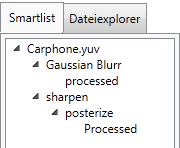
\includegraphics[scale=1]{bilder/projektexplorer.png}
\caption{Projektexplorer}
\label{pExplorer}
\end{figure}
%\nItem{PF} Projektexplorer
%\newline
%Die Anwendung listet alle Referenzvideos und Testvideos des Projekts in einem Projektexplorer auf. Der
% Benutzer kann ein oder mehrere Videos auswählen um auf diesen Filter oder Analysen auszuführen.
% % % % % % % % % % % % % % % % % % % % % % % % % % % % % % % % % % % % % % % % % % % % % % % % % % % % %
%Das ist durch die nächste PF genauer erläutert
%\nItem{PF} Darstellung der Analyseergebnisse als Diagramme
%\newline
%Die Analysedaten werden nach Möglichkeit graphisch durch z.B. Diagramme dargestellt.
% Im Prinzip nicht(komplett ;-) ) falsch, aber die Formulierung gefählt mir nicht und außerdem würden
% wir uns dadurch auf nur eine Art der Visualisierung festlegen.
%\nItem{PF} Darstellung der Analyseergebnisse als Overlay
%\newline
%Analysedaten (z.B. berechnete Unterschiede) werden als Overlay über dem Video eingeblendet.
% Hier eine Alternative
% edit: habe meine Alternative nun auskommentiert da ein paar Zeilen weiter das gleiche in einem 
% besseren Zusammenhang erklärt wird
%\nItem{PF} Die Ergebnisse eines Analysevorgangs werden im Visualisierungsbereich von \gls{OQAT} dargestellt.
%Die Art der Darstellung hängt dabei von der gewählten Analysemetrik ab. Wenn z.B. \gls{mse} als die
%zu verwendende Analysemetrik gewählt wurde wird neben des Differenzvideos(wobei ein Pixel den \gls{mse}
%Wert des jeweiligen Pixels trägt) auch der globale \gls{mse} für das jeweilige Frame und für die gesamte
%Videosequenz dargestellt.
%\nItem{PF} GUI
%\newline
%Die Anwendung unterstützt eine interaktive graphische Benutzeroberfläche mit verschiedenen Sichten, die ein-
% und ausgeblendet werden können. Dabei können Ein- und Ausgabevideos abgespielt, sowie einzelne Frames
%  ausgewählt und visuallisiert werden.
\nItem{PF} Graphische Oberfläche \\
\gls{OQAT} stellt dem Nutzer eine Interaktive Benutzeroberfläche zur Verfügung, die
einzelnen Bestandteile dieser werden im Kapitel \emph{Graphische Oberfläche} näher erläutert.\\
% Gleiches Argument wie oben, das Zeug ist noch nicht sortiert. Da sind pseudoKapitel nur verwirrend.
%\subsubsection{Projektverwaltung}
% Etwas ungenau, sowas haben wir bereits in dem MK. An dieser Stelle muss man also etwas spezifiescher
% werden
%\nItem{PF} Projektverwaltung
%\newline
%Die Anwendung bietet dem Benutzer die Möglichkeit, durch eine \emph{Projekt-Erstellung-Sicht} Projekte
% anlegen, speichern, löschen und verwalten zu können.
\nItem{PF} Projekte anlegen \\
Um \gls{OQAT} verwenden zu können muss der Benutzer ein neues Projekt anlegen oder aber
ein bereits existierendes öffnen. \\
Ein neues Projekt kann entweder über das Hauptmenü, Toolbar oder aber mit Hilfe des sich
im Startfensters befindenden Buttons angelegt werden. Nachdem der Nutzer eine dieser Möglichkeiten
in Anspruch genommen hat, öffnet sich Projekterstellungs-Dialog. In diesem Dialog
muss der Benutzer folgende Daten angeben:
\begin{compactitem}
\item Projektname
\item Ein Pfad unter dem die Projektdaten abgelegt werden sollen. Dieses kann auch leer gelassen werden, 
dann wird ein Defaultpfad verwendet.
\end{compactitem}
% Diese Funktionalität ist in der ">ProjektExplorer"< etwas genauer erläutert worden
%\nItem{PF} Laden von Referenzdateien
%\newline
%Der Benutzer kann durch ein Dialogfenster eine Referenzdatei im YUV-Format in ein Projekt laden, indem er
% den Pfad zu der Datei angibt. Es können mehrere Referenzdateien geladen werden.

%\subsubsection{Portabilität}
%
%\subsubsection{Analyse}

%\nItem{PF} Analysewerkzeugsicht
%\newline
%Alle verfügbaren Analysewerkzeuge werden in dieser Sicht aufgelistet. Der Benutzer kann beliebige Werkzeuge
% markieren und schließlich über einen Button einen Analysedurchlauf für die aus dem Projektexplorer
%  ausgewählten Videodateien starten.
\nItem{PF} MetriList\\
Die \emph{MetriList} enthält alle der Anwendung zur Verfügung stehenden Analysemetriken.
Sobald im SmartTree ein Video und ein gültiges Referenzvideo ausgewählt wurde, darf der Benutzer
eine oder mehrere Metriken auswählen. Eine erfolgreiche Auswahl wird durch das hervorheben des
jeweiligen Eintrags der \emph{MetriList} und einen entsprechenden Vermerk in dem Visualisierungsbereich
gekennzeichnet. Eine Metrik kann erst ausgewählt werden wenn möglicherweise zuvor gewählte Filter,
z.B. durch den Klick auf das entsprechende Symbol aus der Toolbar, bereits angewandt wurden. Versucht
der Benutzer eine Metrik auszuwählen ohne ein Video und Referenzvideo entsprechend markiert zu haben oder
während markierte aber nicht abgearbeitete Filter existieren wird er darauf hingewiesen.

% Muss es hier hin ? In den Musskriterien ist das gleiche drin. -> entweder hier genauer oder aber
% unnötig
%\nItem{PF} Analyse-Metriken
%\newline
%\projektTitel stellt dem Benutzer einige Analyse-Metriken standardmäßig bereit:
%\begin{itemize}
%\item \gls{MSE}
%\item \gls{PSNR}
%\end{itemize}

% Ziemlich wage Formulierung. 
%">..Video werden anhand einer Metrik verglichen.."< Wie genau soll das aussehen ?
%"<..Ergebnisse werden analysiert"< achja ? Wozu und vorallem wie sollen wir die Ergebnisse analysieren ?
% Die Auswertung der Ergebnisse überlassen wir dem Benutzer, wir errechnen die Ergebnisse anhand einer
% Metrik, nicht mehr und nicht weniger. Die Logdatei speichern Geschichte gehört hier nicht ganz hin,
% schließlich hat der Nutzer auch die Möglichkeit solche Daten auch nach dem Durchlauf(nächste Woche..)
% zu exportieren -> Es ist eine eigene Funktionseinheit die beschrieben werden sollte.
% 
%\nItem{PF} Analysedurchlauf
%\newline
%Wenn ein Analysedurchlauf gestartet wird, werden die ausgewählten Videos mittels der ausgewählten
% Analysemetriken verglichen und die Ergebnisse analysiert, bewertet und optional in eine Logdatei
%  gespeichert. Dem Nutzer werden während des Analysedurchlaufs ein Fortschrittsbalken und Statusmeldungen
%   angezeigt. 
% hier ein Gegenvorschlag:
\nItem{PF} Analysevorgang \\
Nachdem der Nutzer eine oder mehrere Metriken aus der \emph{MetriList} und ein
Video samt einem Referenzvideo ausgewählt hat, kann der Benutzer einen Analysevorgang starten. Hat der
Nutzer mehrere Metriken ausgewählt werden diese im Batchverfahren abgearbeitet. Nachdem ein Analysevorgang
beendet wurde, stehen dem Nutzer die Ergebnisse im Visualisierungsbereich zur Verfügung(wurden 
mehrere Metriken angewandt werden diese unter verschiedenen Registerreitern des Visualisierungsbereichs
abgelegt). Die Art der Darstellung der Analyseergebnisse hängt ganz und gar von der Art der gewählten 
Metrik ab. Wenn Beispielsweise die Metrik gls{mse} gewählt wurde wird neben des Differenzvideos(wobei ein
Pixel den \gls{mse} Wert des jeweiligen Pixels trägt) auch der globale \gls{mse} für das jeweilige Frame
und für die gesamte Videosequenz dargestellt.
%%%%%%%%%%%%%%%%%%%%%%%%%%%%%%%%%%%%%%%%%%%%%%%%%%%%%%%%%%%%%%%%%%%%%%%%%%%%%%%%%%%%%%%%%%%%%%%%%%%%%
% ist noch nicht sortiert
%\subsubsection{Verzerrung}
% Eine detailiertere Version davon ist unter PF Filtercontainer zu finden
%\nItem{PF} Filter
%\newline
%Ein Video, welches in ein Projekt eingebunden wurde, kann durch Filter verzerrt werden.Dieses wird
%nach dem Verzerren mit ihrem Referenzvideo verknüpft  Auf solch ein verzerrtes Video kann über den Projektexplorer zugegriffen werden um es ggf. weiter zu verzerren oder zu analysieren.


% Unsinnige unterscheidung zwischen Testsignalen und Filtern
% Das mit den externen Filtern ist eine haarige Angelegenheit
\nItem{PF} Filter-Plugins
\newline
Die Anwendung ist um beliebige Testsignale und Filter in der Form von Plugins erweiterbar.
 Videobearbeitungswerkzeuge (wie z. B. Encoder) kann man auch als externe Filter betrachten und sie als
  Plugins laden, solange sie die Form von ausführbaren Programmen haben und über die Kommandozeile 
angesteuert werden können.

% Bin mir nicht sicher ob es hier nochmal aufgegriffen werden muss
% Bei den Musskriterien ist eine etwas treffendere Beschreibung drin.
% Welchen Zweck wird kantendetektion haben ?
\nItem{PF} Standard-Filter
\newline
Die Anwendung stellt dem Benutzer einige Filter standardmäßig bereit:
\begin{itemize}
\item Weichzeichner
\item Rauschen
\item Farbfilter
\item Blur
\item Schärfe
\item Kantendetektion
\item Emboss
\item Dilatation (Erweiterung)
\item Erosion (Abtragung)

\end{itemize}
%  Etwas kurz geraten, weiter unten ist meine Version
%\nItem{PF} Generierung von Testdateien
%\newline
%Wendet man ausgewählte Filter auf eine Datei an, dann wird eine durch die jeweiligen Filter manipulierte Datei im \gls{glos:YUV} Format generiert, die im Projektordner gespeichert und im Projektexplorer bei den Testvideos aufgelistet wird.
\nItem{PF} Filtervorgang\\
Nachdem der Nutzer einen oder mehrere Filter, gemäß der PF Filtercontainer, markiert hat, kann er
den Filtervorgang, durch den Klick auf das entsprechende Symbol in der Toolbar oder im Hauptmenü,
einleiten. Die Dauer des Filtervorgangs ist Abhängig von der Anzahl der gewählten Filter und der Auflösung
und Länge des gewählten Video aus der Smartlist. Nach einem Filtervorgang wird das neu entstandene Video
als Kindelement, des für den Filtervorgang ausgewähltem Video, aufgeführt.

\subsection{Optionale Funktionalität}
\nItem{PF} Motion Vektoren des .H264 Encoders des \gls{ITEC}\\
Der .H264 Encoder des Instituts gibt, neben der encodierten Videosequenz, auch die verwendeten Motion
Vektoren. \gls{OQAT} kann diese Vektoren im Visualisierungsbereich darstellen.\\
nItem{PF} Drag and Drop\\
Der Projektexplorer ist \emph{Drag and Drop} fähig, d.h. eine gültige Videodatei kann nicht nur über
die Toolbar oder das Hauptmenü hinzugefügt werden sondern darf auch nach dem \emph{Drag and Drop} Prinzip
in die Smartlist eingefügt werden. Das einzubindende Video kann dabei als ein neues Element (ohne
Vaterelement) oder aber als Kindelement eines bereits vorhandenen Videos eingefügt werden.
% So ziehmlich das gleiche ist in unseren WKs zu finden.
%\nItem{PF} Vorschau für Filter
%\newline
%Die Auswirkungen eines Filters oder Testsignals auf ein gewähltes Video werden dem Benutzer als Vorschau an einem Frame veranschaulicht.
% Ich dachte wir haben uns davon verabschiedet.
%
%\nItem{PF} Eingebaute Kommandozeile
%\newline
%Der Benutzer hat die Möglichkeit, durch eine Kommandozeile Argumente an die Anwendung übergeben zu können.
% Eine ähnliche Beschreibung ist in den Musskriterien verzeichnet
%\nItem{PF} Logdatei
%\newline
%Es gibt die Option, eine Logdatei für einen Analysevorgang zu erstellen. In der Logdatei sollen im Rahmen
% des jeweiligen Analysevorgangs ausgeführte Operationen sowie erhaltene Ergebnisse in Textformat
%  chronologisch aufgelistet werden. Die Auswahl, welche Arten von Operationen und Ergebnissen in der
%   Logdatei gespeichert werden sollen, steht dem Benutzer zur Verfügung.





\chapter{Produktdaten}
Ein Projekt fasst folgende Daten zusammen:
	\begin{itemize}
		\item Projektname und -beschreibung
		\item Dateipfad zu Referenzvideos als .yuv-Dateien (optional - es ist auch möglich nur mit generierten
		 Testsignalen zu arbeiten)
		\item Reihenfolge und Parameter der angewendeten Filter oder Testsignale
	        \item Testvideos als .yuv-Dateien, die durch Filter aus den Referenzvideos oder Testsignalen
	         generiert wurden
	        \item Angaben (Pfad, Parameter) zur Ansteuerung des zu testenden Videobearbeitungswerkzeugs 
	        oder Encoders (optional)
		\item Ergebnisse der Analysedurchläufe, abhängig von der gewählten Metrik
		\item Errorlogs
	\end{itemize}
Die Einstellungen werden in einer XML-Datei gespeichert. Analyse-Ergebnisse werden in separaten Dateien
 gespeichert. Die generierten Testvideos werden vom Programm im Projektunterordner "Testvideos" abgelegt.


% brauchen wir auch eine Beschreibung des YUV-Format?
% Ja !

\chapter{Qualitätsbestimmungen}

\begin{itemize}
\item Die GUI soll falsche Benutzereingaben weitestgehend vermeiden.
\item Fehlerhafte Eingaben für Pfad, Frames per second, Filter und Analysemetriken werden vom Programm nicht angenommen und der Benutzer wird gefordert, sie zu korrigieren.
\item Ein Filter- oder Analysevorgang findet nur für gültige YUV-Dateien statt, d.h. wenn eine YUV-Datei nicht gelesen werden kann, stürzt das Programm nicht ab und gibt eine entsprechende Fehlermeldung aus.
%Der Nutzer sollte ohne lange Einarbeitungsphase das Programm bedienen können.
\item \projektTitel wird Benutzern eine Hilfe, in Form von Tooltipps und einer kurzen Einleitung die wichtigsten Programmfunktionen anbieten.
\item Die Anwendung wird ausführlich getestet.
\end{itemize}
\include{inhalt/gui}
\chapter{Globale Testfälle}
\section{Testfälle}
\setcounter{counterKriterien}{0}

%veraltet => neu schreiben
------------*

\nItem{T} Projekt erstellen, speichern und laden
\nItem{T} Projekt bearbeiten, speichern und laden
\nItem{T} Projekt auf anderem Rechner öffnen

\nItem{T} Filter auswählen ohne Video ausgewählt zu haben - Fehlermeldung
\nItem{T} Filter auswählen, Vorschau betrachten
\nItem{T} Filter anwenden, generierte Video-Datei überprüfen
\nItem{T} Filter-Einstellungen verändern
\nItem{T} Mehrere Filter auf ein Video anwenden, Reihenfolge verändern

\nItem{T} Analysemetrik auswählen ohne zwei Videos ausgewählt zu haben - Fehlermeldung
\nItem{T} Analyse starten ohne Metrik auszuwählen - Fehlermeldung
\nItem{T} Analyse durchführen, Ergebnisse anzeigen
\nItem{T} Analyseergebnisse speichern und laden
\nItem{T} Analyseergebnisse exportieren (csv)

\nItem{T} GUI Funktionalität




\section{Testszenarien}
\setcounter{counterKriterien}{0}

%Projekt erstellen
%Bestehendes Projekt öffnen
%Filter anwenden
%Makrofilter erstellen
%Analyse
%alte Analysedaten anzeigen

\nItem{TS} Neues Projekt erstellen\\
\begin{enumerate}
\item \dAU startet \projektTitel.
\item Der Wilkommensbildschirm öffnet sich.
\item \dAU klickt auf den \emph{neues Projekt erstellen} Button.
\item Ein Projekt Erstellungsdialog wird geöffnet.
\item \dAU trägt einen Projekt Titel, eine kurze Beschreibung ein und bestätigt den Vorgang.
\item \dAU klickt auf den Dateiexplorer und wählt \emph{carphone.yuf} mit einem Rechtklick aus. Aus dem erscheinenden Dialog wählt er die \emph{Ressource hinzufügen} Option aus.
\item Das Video wird nun im Projektexplorer angezeigt.
\item \dAU beendet das Programm, da sein Ziel erreicht ist.
\end{enumerate}


\nItem{TS} Bestehendes Projekt öffnen\\ %Filter anwenden/Makrofilter erstellen
\begin{enumerate}
\item \dAU startet \projektTitel
\item Der Willkommesnbildschirm öffnet sich.
\item \dAU wählt aus der Liste seiner zuletzt geöffneten Projekten das \emph{H264Test} Projekt aus.
\item \dAU klickt auf das \emph{carphone.yuf} Video im Smarttree.
\item \dAU wählt den Weichzeichner aus der Filterliste aus.
\item \dAU erhöht die stärke des Weichszeichners und fügt es der Warteliste der Anzuwendenden Filter hinzu.
\item \dAU wählt den Scharfzeichner aus der Filterliste aus und fügt es zur Warteliste der anzuwendenden Filter hinzu. 
\item \dAU schiebt den Scharfzeichner vor den Weichzeichner in der Warteliste.
\item \dAU speichert die Reihenfolge unter dem Namen \emph{ScharfWeich} ab.
\item \dAU klickt auf Filter anwenden.
\item Das Video wird im \emph{smarteTree} als Kindelement des \emph{carphone.YUF} aufgelistet.
\item  \dAU beendet \projektTitel.
\end{enumerate}

\nItem{TS} Analyse
\begin{enumerate}
\item \dAU startet \projektTitel.
\item öffnet das \emph{H264Test} Projekt.
\item \dAU wählt im Dateiexplorer die \emph{carphoneH264encoded.YUF} und fügt diese als Kindelement des \emph{carphone.yuv} Video (im emph{smartTree}) hinzu.
\item \dAU wählt die \emph{PSNR} Metrik aus der Metrikenliste aus.
\item \dAU markiert das \emph{carphone.yuv} Video aus dem \emph{smartTree} als Referenzvideo und \emph{carphoneH264encoded.YUF} als das zu analysierende Video.
\item \dAU startet die Analyse durch einen Klick auf das ensprechende Symbol der Toolbar.
\item \dAU wartet bis der Analysevorgang beendet wurde.
\item \dAU schaut sich die Ergebnisse der Analyse an und gibt eine Beschreibung an die er zusammen mit den Analyseergebnissen abspeichert um auch später auf diese zurückgreifen zu können.
\item \dAU schließt das Programm.
\end{enumerate}

\chapter{Systemmodelle}

\section{Szenarien}

\section{Anwendungsf"alle}

\section{Objektmodell}

\section{Dynamische Modelle}

\section{Grafische Benutzerschnittstelle}
\include{inhalt/entwicklungsumgebung}

%Glossar ausgeben
\printglossary[style=altlist,title=Glossar]

%Abkürzungen ausgeben
\deftranslation[to=German]{Acronyms}{Abkürzungsverzeichnis}
\printglossary[type=\acronymtype,style=long]

%Symbole ausgeben
\printglossary[type=symbolslist,style=long]

\end{document}